\section{Background of the Study}

Road accidents has become one of the most prevalent cause of death in the Philippines wherein 26\% of it was caused by driver errors (Tamayo, A., 2009). Driver error includes driver fatigue, the proposed thesis aims to create a device that would alert the driver in time to help in prevention of such accidents. One way of determining whether a driver is feeling drowsy is by observing eye behaviour. One of the significant eye metrics that determines whether a driver is feeling drowsy is the frequency of eye closure exceeding one second whereas shorter ones are considered as blinks (Verwey \& Zaidel, 2000). The researchers intend to do a similar thing with regards to evaluating driver fatigue by observing the eyes. In addition to the eye metrics to be used for driver fatigue detection, head pose estimation will also be an additional parameter using RGB-D camera. As compared to the conventional RGB camera, the advantage of an RGB-D camera is its capability of capturing depth which helps in 3-D representations and modelling. These cameras augment the usual images with its depth information. The augmentation happens in per-pixel basis. Along with the RGB image captured from the camera, the eye parameters, the depth data (head pose)  will be used in order to develop an algorithm for driver fatigue detection.

The eye metrics to be used in this research are blink rate and blink duration. The blink rate refers to the number of blinks that has occurred within a given time period and the blink duration refers to the time where the eyes are in the close state before entering the open state. On a normal condition, the average of the blink duration of a human would range from 100-400ms and exceeding 1000ms is considered as a microsleep (Schiffman, H., 1990). Whereas the normal blink rate would range from 0.33blinks/s to 0.25blinks/s (Nakano, T., et al., 2013). It can be seen that as the number of blinks increases over a period of time, the higher the blink rate and the lower the number of blinks over a period of time, the lower the blink rate.
One past study presents the use of Kinect as the RGB-D camera to track eye gazing by using the algorithm from the thesis Eye-Model-Based Gaze Estimation by RGB-D Camera (Jianfeng \& Shigang, 2014). The Kinect sensor is able to acquire the pose and 3D position of the head. In past researches, RGB camera can be used for detection of driver drowsiness by utilization of image processing (Ballesteros, P., et al, 2012). In this past research in order to come up with a conclusion that the driver is drowsy and an alarm is needed to wake up the driver, the authors based it on the eye behavior and frequent nodding of the driver.



\newpage
\section{Prior Studies}

\begin{table}[!htb]
	\caption{List of Previously Done Studies}
	\begin{tabular}{|l|l|l|l|}
		\hline
		\multicolumn{1}{|c|}{\begin{tabular}[c]{@{}c@{}}Past Study\\ (Title, Author)\end{tabular}}                                                                        & \multicolumn{1}{c|}{Brief Description}                                                                                                                                                                                & \multicolumn{1}{c|}{Advantages}                                                                                                                                                                                                                                                                                                                      & \multicolumn{1}{c|}{Improvements of Our Study}                                                                                                                                                                                        \\ \hline
		\begin{tabular}[c]{@{}l@{}}Real-Time \\ System for \\ Driver Fatigue \\ Detection by \\ RGB-D Camera \\ (Zhang, L., Liu, \\ F. \& Tang, J., \\ 2015)\end{tabular} & \begin{tabular}[c]{@{}l@{}}Driver fatigue \\ |detector that \\ makes use of \\ an RGB-D \\ sensor to \\ measure eye\\ state parameters\\ and head \\ pose in real-time\end{tabular}                                   & \begin{tabular}[c]{@{}l@{}}1.Real-Time \\ Detection\\ 2.Outputs \\ are not based \\ on one \\ parameter only\\ 3.Utilizes an \\ RGB-D sensor\\ for its depth \\ data that \\ serves as extra \\ evidence for \\ parameter \\ detection\\ 4.Using WLBP \\ (Weber Local \\ Binary Pattern), \\ the accuracy \\ of detection \\ is at 82\%\end{tabular} & \begin{tabular}[c]{@{}l@{}}1.The system will be trained \\ and calibrated using an \\ existing database\\ 2.Intensity images will not \\ be used as inputs to the \\ system in order to tolerate \\ illumination changes\end{tabular} \\ \hline
		\begin{tabular}[c]{@{}l@{}}Eye Tracking \\ for Everyone \\ (Krafka, K., \\ et.al, 2016)\end{tabular}                                                              & \begin{tabular}[c]{@{}l@{}}A convolutional \\ neural network, \\ iTracker, was \\ designed and \\ implemented for \\ eye tracking \\ while utilizing \\ GazeCapture \\ which is a \\ large-scale dataset\end{tabular} & \begin{tabular}[c]{@{}l@{}}1.Utilizes a \\ large-scale \\ dataset.\\ 2.Crowd\\ sourcing \\ was the \\ method of \\ data collection\\ 3.Robust eye \\ state tracking \\ due to proper \\ calibration\end{tabular}                                                                                                                                     & \begin{tabular}[c]{@{}l@{}}1.Reliability will be \\ improved by adding head \\ pose parameters\\ 2.High variability will be \\ encouraged to reduce the \\ number of calibration that \\ are necessary\end{tabular}                   \\ \hline
	\end{tabular}
\end{table}

\begin{table}[!htb]
	\begin{tabular}{|l|l|l|l|}
	\hline
\begin{tabular}[c]{@{}l@{}}Drowsy Driver \\ Identification \\ Using Eye \\ Blink Detection \\ (Ahmad, R. \\ \& Borole, J., \\ 2015)\end{tabular}                  & \begin{tabular}[c]{@{}l@{}}A non-intrusive \\ machine \\ vision-based \\ concept was used \\ to design and\\ implement a \\ drowsiness \\ detection system \\ based on the \\ blink rate\end{tabular}                 & \begin{tabular}[c]{@{}l@{}}1.All possible \\ actions are \\ considered \\ and outputs are \\ generated \\ accordingly.\\ 2.The \\ parameters are \\ not limited to \\ the eyes.\\ 3.Driver’s \\ attention is also\\ considered\\ 4.Drowsiness \\ detection \\ accuracy is \\ currently at 95\% \\ with processing \\ time of 2 sec.\end{tabular}     & \begin{tabular}[c]{@{}l@{}}Additional eye state \\ parameter will be introduced \\ in our study which is the \\ blink duration\end{tabular}                                                                                           \\ \hline
\begin{tabular}[c]{@{}l@{}}Real Time \\ Implementation \\ of Eye Tracking \\ System Using \\ Arduino Uno \\ Based Hardware \\ Interface \\ (Venugopal, B. \\ \& D’souza, D., \\ 2016)\end{tabular} & \begin{tabular}[c]{@{}l@{}}Implemented a \\ system using \\ Arduino Uno and\\ Zigbee wireless \\ device for eye \\ tracking and \\ movement \\ estimation\end{tabular}                                                             & \begin{tabular}[c]{@{}l@{}}1.Has movement \\ detection feature\\ 2.Transmission of \\ data is wireless\end{tabular}                                                                                                                                                                                                                                  & \begin{tabular}[c]{@{}l@{}}1.An additional device will \\ not be required because the \\ microcontroller to be used \\ has built-in wireless \\ capabilities.\end{tabular}                                                                                                                                           \\ \hline
\begin{tabular}[c]{@{}l@{}}Eye Gaze \\ Tracking Based \\ Driver \\ Monitoring\\ System (Mavely, \\ A., Judith, J. \& \\ Kuruvilla, S., \\ 2017)\end{tabular}                                       & \begin{tabular}[c]{@{}l@{}}Eye gaze tracking \\ system for driver\\ drowsiness was \\ implemented using \\ Raspberry Pi.\end{tabular}                                                                                              & \begin{tabular}[c]{@{}l@{}}1.Notification \\ using audio \\ and vibration \\ on the steering \\ wheels.\\ 2.Accuracy is \\ high in any light \\ conditions.\\ 3.Less expensive\end{tabular}                                                                                                                                                          & \begin{tabular}[c]{@{}l@{}}1.Different levels of \\ drowsiness will be \\ analyzed for different \\ alarm notifications\\ 2.Drowsiness detection \\ will also be based on \\ head pose parameters \\ such as the tilting of \\ the head.\end{tabular}                                                                \\ \hline
	\end{tabular}
\end{table}
\begin{table}[t]
	\begin{tabular}{|l|l|l|l|}
		\hline
\begin{tabular}[c]{@{}l@{}}Face and Head \\ Detection for a \\ Real-Time \\ Surveillance \\ System (Ishii, Y., \\ Hongo, H., \\ Yamamoto, K. \\ \& Niwa, Y., \\ 2004)\end{tabular}                 & \begin{tabular}[c]{@{}l@{}}Two classifiers \\ were used in \\ order to detect \\ the face and \\ head effectively \\ which is then \\ implemented using \\ a PC and run at \\ approximately \\ 10fps for VGA \\ input\end{tabular} & \begin{tabular}[c]{@{}l@{}}1.Head detection \\ is at 87.2\% and \\ its reliability is \\ at 83.6\%\\ 2.Makes use of \\ Four Directional \\ Features for \\ robust detection \\ of patterns\end{tabular}                                                                                                                                              & \begin{tabular}[c]{@{}l@{}}1.False alarms will be \\ greatly reduced because \\ the distance between the \\ sensor and the subject is \\ ideal\\ 2.Training procedure for\\ the system will be\\ improved because of the \\ large-scale dataset\end{tabular}                                                         \\ \hline
	\end{tabular}
\end{table}
\section{Problem Statement}


One of the reasons for fatal traffic accidents is driver drowsiness. The researchers aim to detect driver drowsiness with three parameters: blink rate, blink duration, and head pose estimation. These three parameters will be integrated to be able to come up with the final evaluation which could then display the level of drowsiness of the driver through the use of indicator or alert the driver if the level of drowsiness reached the worst level. It will be based on the number of times the driver has nodded and if the driver’s head deviates from its normal position for a long time. The problem to be resolved in this thesis is the accuracy of getting a correct evaluation of driver fatigue due to its dependency on acquiring the three parameters needed. The acquisition of the blink duration, blink rate, and head pose should also have a high accuracy so that false alarms could be avoided. 



\section{Objectives}


\subsection{General Objective(s)}
The main objective of the thesis is to design and implement a system that will detect the level of fatigue of the driver and to alarm the driver once the level of fatigue reached a certain level not suitable for driving.

\subsection{Specific Objectives}

\begin{enumerate}
	
	\item To develop an algorithm for detection of driver fatigue based on parameters such as blink duration, blink rate, and head pose estimation
	
	\item To integrate eye state parameters and head pose estimation for determining the final evaluation of the level of driver fatigue
	
	\item To utilize a microcontroller such that data acquired from the RGB-D sensor will be processed for driver fatigue evaluation
	
	\item To create an alarm system, consisting of an indicator and a speaker, that will notify the driver of their level of drowsiness
	
	\item To achieve at least 95\% accuracy in determining the level of drowsiness: Alert, Low Alertness, Drowsy, and Sleeping
	
	
\end{enumerate}



\section{Significance of the Study}

Eye tracking is very significant because almost every work and action require visual information; Eye tracking is able to track the behavior of the human eyes wherein it could observe how the human eye reacts in different situations. Some of the capabilities of eye trackers include detecting drowsiness, consciousness, and other mental states. The integration of these eye trackers to available electronic devices such as computers and mobile phones helps in analysis of consumer’s behavior and may lead to further technological advancements. Eye tracking technology also helps in researches and designs of fields including auto motives, medical, defense, and entertainment industries. These applications progress as time passes by wherein these progressions may root from the technology and research that this paper will provide.

In order to make the driver fatigue detection system become more accurate, it is also important to know the head position of the driver. Knowing the head position will enable the researchers to obtain more visual information regarding drowsiness level. The simplest of actions such as head swaying and nodding is already enough to know if the driver is exhausted. 
One example to know if the driver is exhausted includes the head not in the frontal position for an extended period of time. This means that the head is already tilted to one side or nodding off.

By understanding the user’s eye and head behavior, new safety and security measurements may be designed. In addition, there will be improvements on existing work based on data gathered from eye and head movements. The beneficiaries of this study include the user, the society and industries that make use of visual data for improvements, and future researchers as well. The user and the industries that continue to improve their products and devices help each other in such a way that the safety, security, and satisfaction of the users will be achieved given that their visual data and gaze patterns will be carefully analyzed by different industries. This study also helps in improving and testing of existing algorithms for eye tracking and head pose estimation. Therefore, this study will be of great help to future researchers that will engage and tackle this topic because eye tracking and head pose estimation is important and significant in this modern age. 




\section{Assumptions, Scope and Delimitations}


\subsection{Assumptions}
\begin{enumerate}
	
	\item The existing dataset to be used upon developing the system will come from a research study about eye tracking conducted by Krafka et. al. (2016) from Massachusetts Institute of Technology (MIT) 
	
	\item The RGB-D camera will have a difficulty in detecting the eyes if the person being evaluated has little eye openings 
	
	\item The device will treat head movements as nods or head tilts due to road humps or cracks which can affect the accuracy and reliability of the system
	

	
\end{enumerate}

\subsection{Scope}
\begin{enumerate}
	
	\item The device can measure the blink rate and blink duration of the eyes as additional parameters in determining whether the driver is drowsy or not.
	
	\item It can also detect driver fatigue by using head pose estimation
	
	\item The device should be able to detect and classify the level of drowsiness of the driver.
	
	
	\item Evaluation of driver awareness using the device is still accurate even on low light conditions
	
	\item The prototype will be tested in a laboratory setting and in a vehicle
	
	\item The size of the RGB-D sensor to be placed at the dashboard of the vehicle will not exceed the 4 inches height allowance of the distracted driving law
	
	
\end{enumerate}

\subsection{Delimitations}
\begin{enumerate}
	
	\item The thesis will only be tested on standard cases, these does not include people with glasses, face or eye disorders, and eye irritation
	
	
	\item The device will be placed inside closed/private vehicles to maximize the effectiveness of the alarm system
	
	\item The system will not be interfaced with the computer box of the vehicle
	
\end{enumerate}

\section{Description and Methodology}

Visual data gathered by the RGB-D camera will be used to study and analyze the eye movements and head pose of the driver. Moreover, there will be an alarm system when the camera detects driver fatigue which is not suited for driving a vehicle. 

The head pose is estimated using the RGB-D camera and a head coordinate system is generated. If the system has detected that the driver has deviated from the reference or the normal position of the head for a certain time while the eye parameters are being monitored, then the device will evaluate if the driver has nodded off and an alarm will turn on to wake up the driver from sleeping. The head pose of the driver will serve as a basis for evaluation of driver fatigue along with the gathered blink rate and blink duration. The different head poses based from the estimated head pose results are given below in Figure 1.1.
\newline

\begin{figure}[ht]
	\centering
	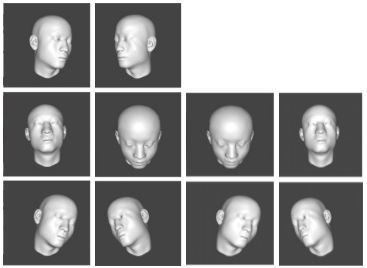
\includegraphics[scale=1]{figheads}
	\caption{Different head poses based from estimated head pose results (Liu, F. et. al., 2015)}
\end{figure}


\begin{table}[!htb]
	\caption{Evaluation of level of Drowsiness}
	\begin{center}
	\begin{tabular}{|c|c|}
		\hline
		\textbf{Level of Drowsiness} & \textbf{Description}                                                                                             \\ \hline
		Awake                        & \begin{tabular}[c]{@{}c@{}}Normal blink rate (0.25 - 0.33 blink/s)\\Normal blink duration (100-400ms)\\Or \\Low blink rate (less than 0.25blink/s) \\Normal blink duration(100-400ms) \end{tabular}         
		\\ \hline
		Low Alertness                & \begin{tabular}[c]{@{}c@{}}Normal blink rate (0.33blink/s - 0.25blink/s)\\Long blink duration(400ms - 1s)\\Or\\Low blink rate (lower than 0.25blink/s)\\Long blink duration(400ms - 1s) \end{tabular} 
		\\ \hline
		Drowsy                       & \begin{tabular}{@{}c@{}}High blink rate (0.33blink/s)\\Long blink duration (400ms-1s)\\Or\\Normal blink rate\\Long blink duration (400ms - 1s)\end{tabular} 
                                                                                 
		\\ \hline
		Sleepy                       & \begin{tabular}[c]{@{}c@{}}Low Blink Rate (less than 0.25blink/s)\\Very long Blink Duration (greater than 1s)\end{tabular}
        \\ \hline
		
	\end{tabular}
	\end{center}
	\end{table}
	
\newpage
It is evaluated into four levels such as Awake, Low Alertness, Drowsy, and Sleepy. Each level of drowsiness will have an indicator and if the driver is evaluated as sleepy or drowsy an alarm will sound off to warn the driver. 
\newpage
\begin{center}
\begin{figure}[ht]
	\centering
	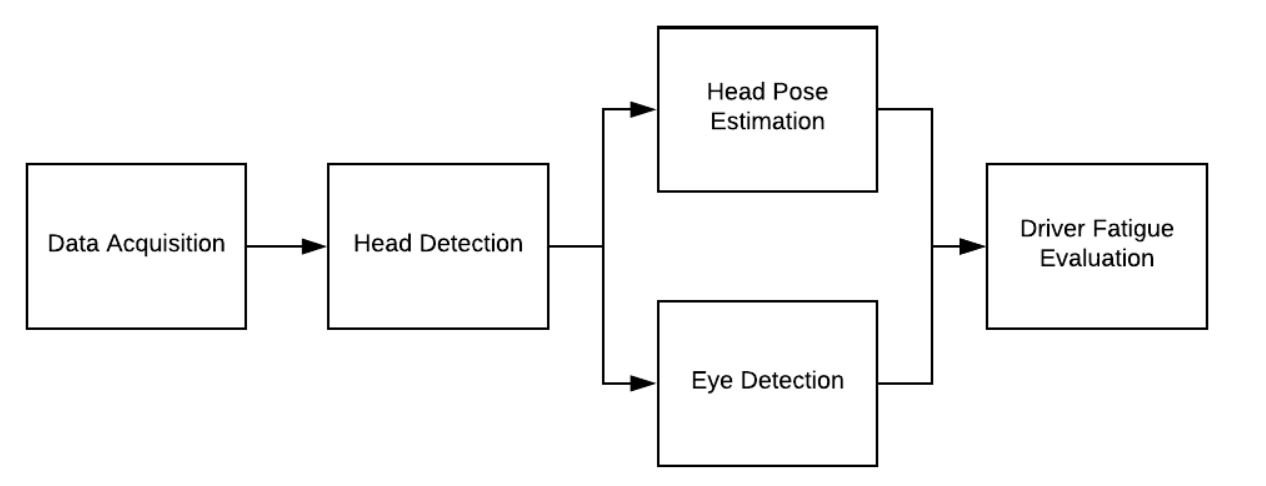
\includegraphics[scale=0.5]{flow}
	\caption{General Framework of Driver Fatigue Evaluation System}
\end{figure}
\end{center}


The RGB-D camera is continuously taking a video of the face of the driver and frames will be captured. If the face and head is now detected, the edges of the faces will then be taken in order to find the location of the eyes. After eye detection, blink rate, blink duration, and head pose was calculated for evaluation of driver fatigue. The algorithm to be used for the evaluation of fatigue will be classifiers. Some examples that can be used as classifiers are machine learning algorithms, fuzzy logic, etc. 


\begin{center}
	\begin{figure}[ht]
		\centering
		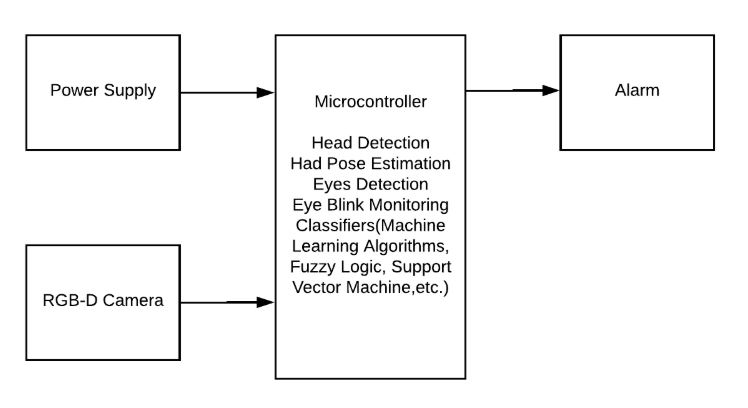
\includegraphics[scale=0.8]{blocks}
		\caption{Proposed Block Diagram of Driver Monitoring System}
	\end{figure}
\end{center}
\newpage 
The RGB-D Camera will serve as the sensor for the eye movements and head movements. The microcontroller will then process the data acquired by the RGB-D. If the system has detected that the driver’s fatigue level is high, the alarm system will turn on and notify the driver. 
\section{Overview}

\subsection{Gantt Chart}
\newpage
The following figures shown below is the individual gantt chart of the researchers:

\begin{figure}[!htb]
	\centering
	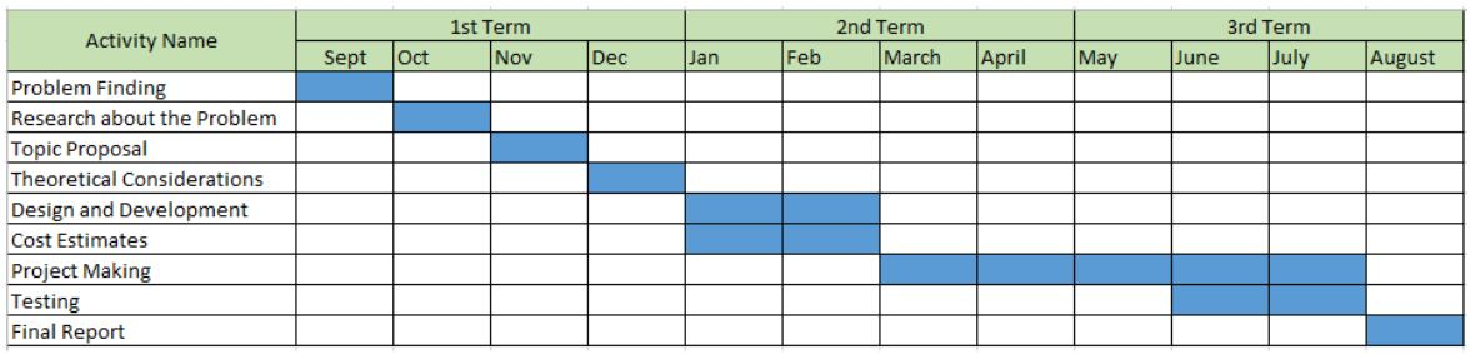
\includegraphics[scale=0.25]{gantt1}
	\caption{Gantt Chart of Guevarra}
\end{figure}
\begin{figure}[!htb]
	\centering
	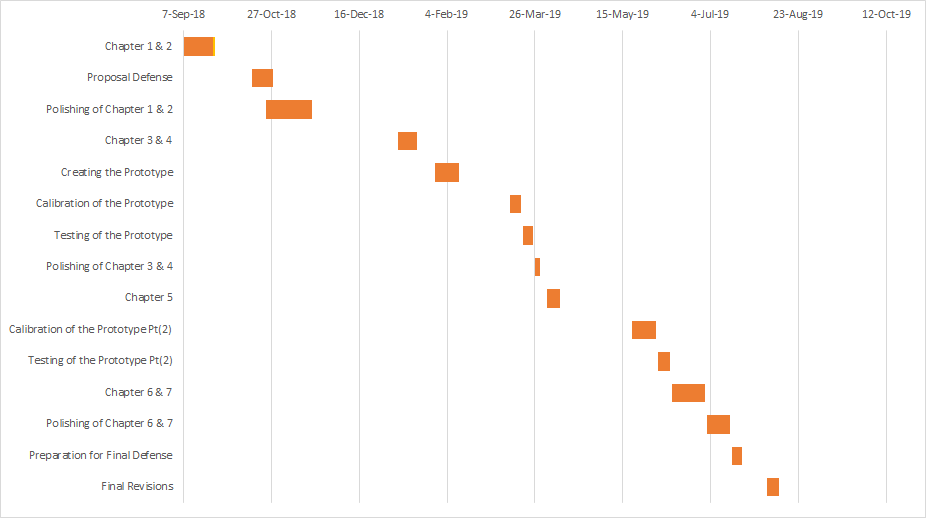
\includegraphics[scale=0.6]{gantt2}
	\caption{Gantt Chart of Hernandez}
\end{figure}
\begin{figure}[!htb]
	\centering
	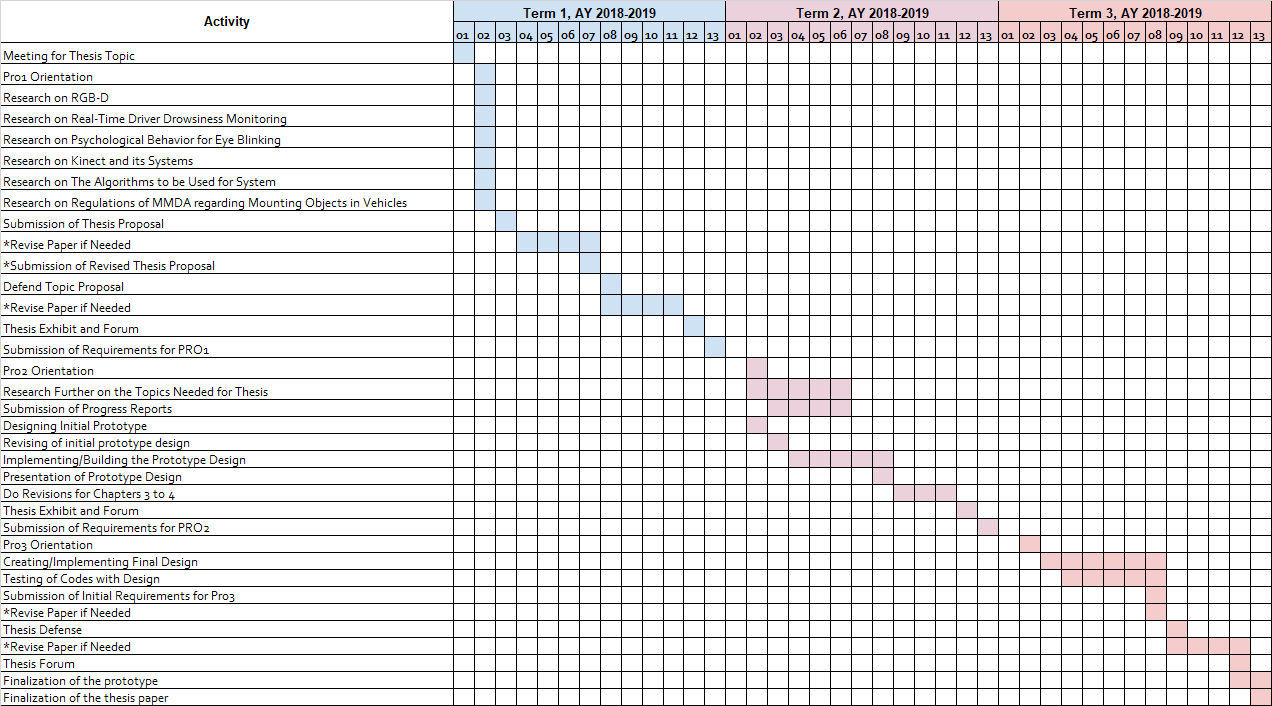
\includegraphics[scale=0.42]{gantt3.png}
	\caption{Gantt Chart of Lagman}
\end{figure}
\begin{figure}[!htb]
	\centering
	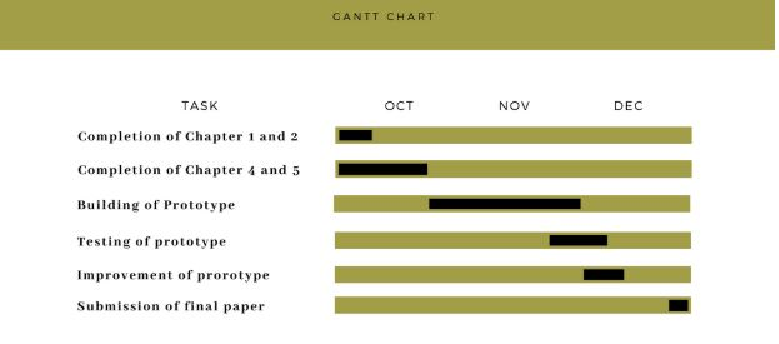
\includegraphics[scale=0.6]{gantt4}
	\caption{Gantt Chart of Villanueva}
\end{figure}
\newpage
\newpage
\subsection{Estimated Work Schedule and Budget}
\begin{table}[!htb]
	\caption{Price List of Materials to be Used}
	\centering
	\begin{tabular}{|c|c|}
		\hline
		Materials & Estimated Price(in PHP) \\
		\hline
		RGB-D Sensor & Php10,000-20,000 \\
		\hline
		Microcontroller & Php450-25k \\
		\hline
		Laptop & Php15k-100k \\
		\hline
		Total Price & Php25k-140k \\
		\hline
	\end{tabular}
\end{table}